\bigskip

\item Which of the following is a graph of $y=\log_2 x$?
\bigskip


% (a)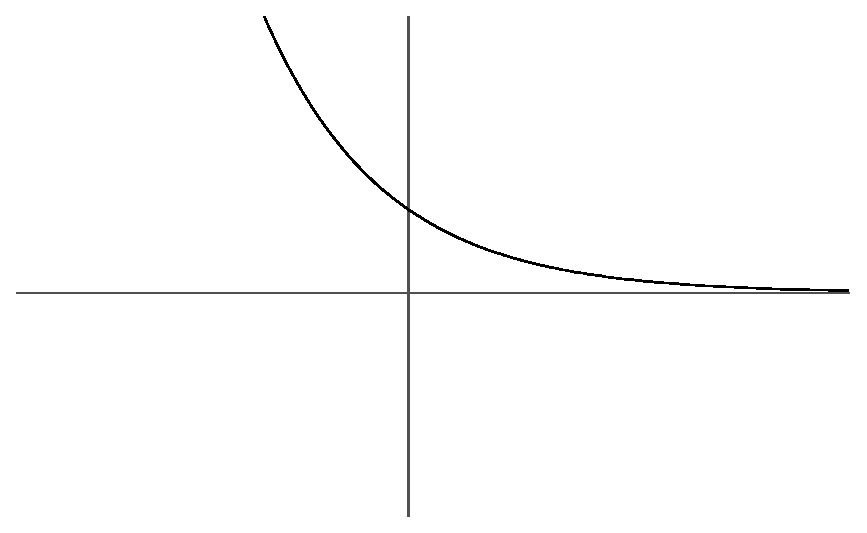
\includegraphics[height=90pt]{SVC.01.04.026a.eps}(b)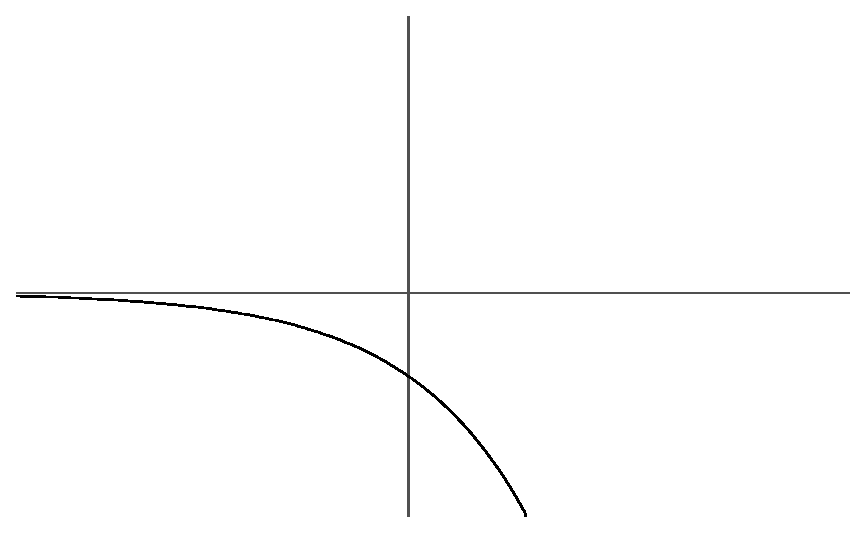
\includegraphics[height=90pt]{SVC.01.04.026b.eps}\\
% (c)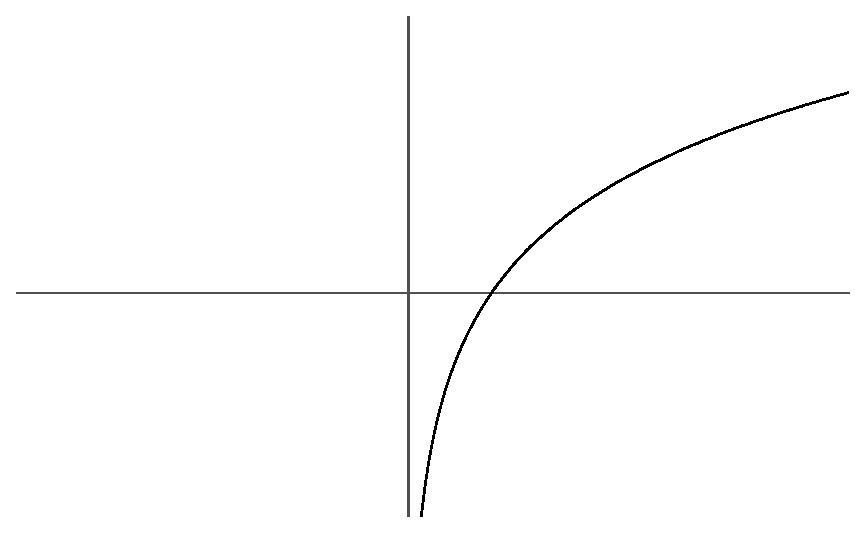
\includegraphics[height=90pt]{SVC.01.04.026c.eps}(d)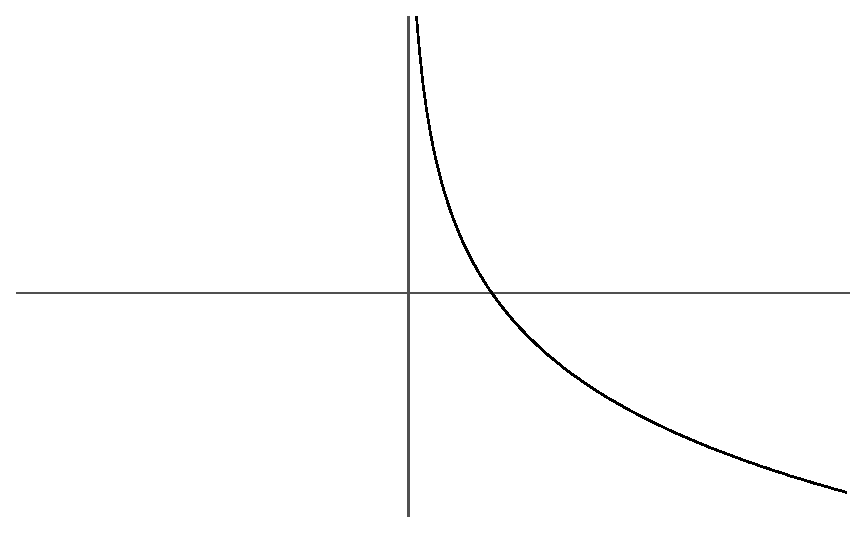
\includegraphics[height=90pt]{SVC.01.04.026d.eps}

\begin{tikzpicture}
        \begin{axis}[axis lines=center, xlabel={$x$}, ylabel={$y$}, xmin=-3, xmax=3,
                ymin=-3, ymax=3, xtick=\empty, ytick=\empty, yticklabels={},
            xticklabels={}, title={Plot (a)}]
                \addplot[color=blue, very thick,samples=100] {(1/2)^x};
            \end{axis}
        \end{tikzpicture}
    \begin{tikzpicture}
        \begin{axis}[axis lines=center, xlabel={$x$}, ylabel={$y$}, xmin=-3, xmax=3,
                ymin=-3, ymax=3, xtick=\empty, ytick=\empty, yticklabels={},
            xticklabels={}, title={Plot (b)}]
                \addplot[color=blue, very thick,domain=-3:3,samples=100] {-1*2^x};
            \end{axis}
        \end{tikzpicture}\\
    \begin{tikzpicture}
        \begin{axis}[axis lines=center, xlabel={$x$}, ylabel={$y$}, xmin=-3, xmax=3,
                ymin=-3, ymax=3, xtick=\empty, ytick=\empty, yticklabels={},
            xticklabels={}, title={Plot (c)}]
                \addplot[color=blue, very thick,domain=-3:3,samples=100] {ln(x)/ln(2)};
            \end{axis}
        \end{tikzpicture}
    \begin{tikzpicture}
        \begin{axis}[axis lines=center, xlabel={$x$}, ylabel={$y$}, xmin=-3, xmax=3,
                ymin=-3, ymax=3, xtick=\empty, ytick=\empty, yticklabels={},
            xticklabels={}, title={Plot (d)}]
                \addplot[color=blue, very thick,domain=-3:3,samples=100] {-1*ln(x)/ln(2)};
            \end{axis}
        \end{tikzpicture}
%by Project MathVote

